\subsection{Case05 - Broadcast}
\label{xdp_wifi_case05}
\vspace{0.3cm}
Por último, en este caso de uso exploraremos la capacidad de broadcast de \gls{xdp} en entornos inalámbricos. Por ello se ha intentado replicar un escenario básico de broadcast en un escenario inalámbrico. Se ha planteado hacer uso de la herramienta arping para emular una resolución ARP, generando ARP-Request, estos llevan su MAC destino todo a \texttt{FF:FF:FF:FF:FF:FF} y su dominio de difusión englobaría todos aquellos nodos de la red que operen hasta capa 2.\\
\par

% figura escenario
\begin{figure}[ht]
    \centering
    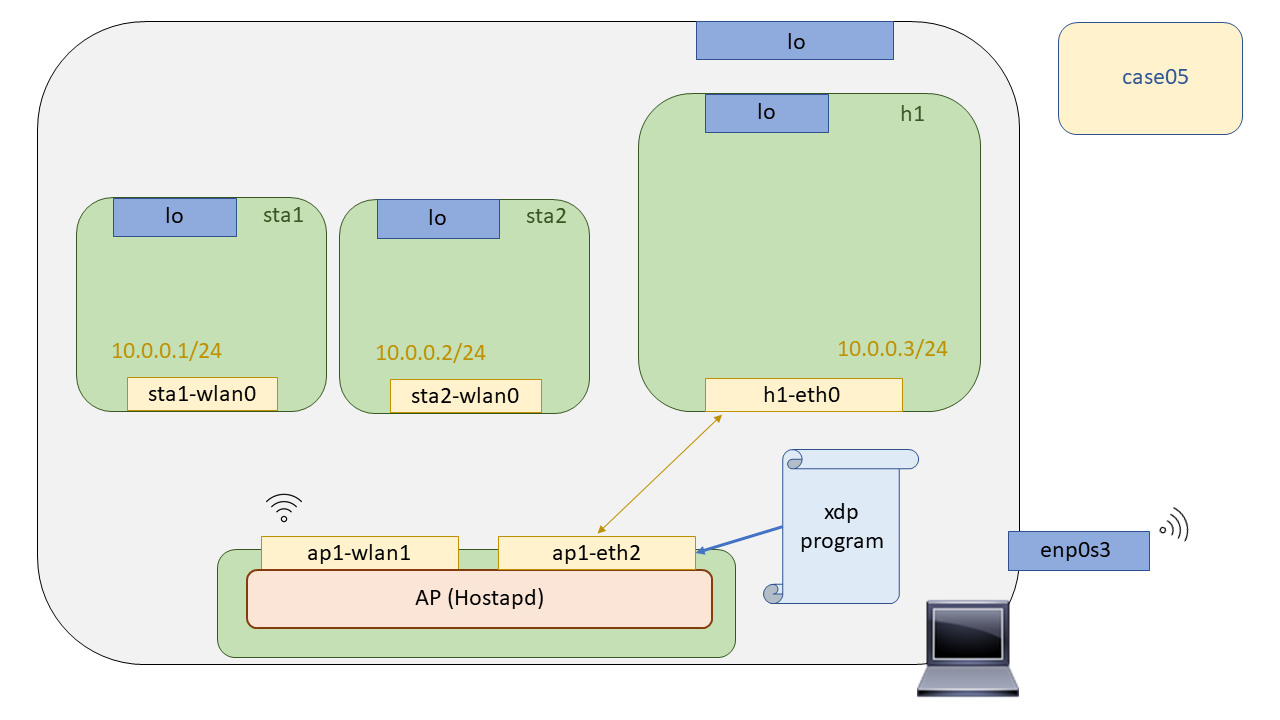
\includegraphics[width=16cm]{archivos/img/dev/xdp-wifi/case05/scenario.png}
    \caption{Escenario inalámbrico del Case05 - XDP}
    \label{fig:case05_xdp_wifi_scenario}
\end{figure}


El escenario propuesto para este caso de uso se puede apreciar en la figura \ref{fig:case05_xdp_wifi_scenario}. Este estaría compuesto de dos estaciones wireless conectadas a un punto de acceso, sobre el cual irá toda la lógica XDP, y por último, un host desde el que podremos empezar las resoluciones ARP para ver así su difusión en un medio wireless. En este caso, sí es viable hacer Broadcast debido a la condición de un medio inalámbrico, ya que al tener una única interfaz \textit{wireless} para interconectar todos los nodos inalámbricos, solo sería necesario enviar el paquete con MAC destino todo a \texttt{FF:FF:FF:FF:FF:FF} para lograr el Broadcast. 


\vspace{0.5cm}
\textbf{Compilación}\\
\par

Para compilar el programa \gls{xdp}, al igual que en casos de uso anteriores, se ha dejado un Makefile preparado en este directorio. Por lo tanto, para compilarlo únicamente hay que seguir las indicaciones del bloque \ref{code:case05_xdp_wifi_compilacion}.

\begin{lstlisting}[language= bash, style=Consola, caption={Compilación programa XDP - Case05},label=code:case05_xdp_wifi_compilacion]
    # En caso de no haber entrado en el directorio asignado del caso de uso
    cd TFG/src/use_cases/xdp-wireless/case05
    
    
    # Hacemos uso del Makefile suministrado 
    sudo make
\end{lstlisting}
\vspace{0.5cm}

Si tiene dudas sobre el proceso de compilación del programa \gls{xdp} le recomendamos que vuelva al case02 (\gls{xdp} - Cableado \ref{xdp_ether_case02}) donde se hace referencia al \textit{flow} dispuesto para la compilación de los programas \gls{xdp}.\\
\par



\vspace{0.5cm}
\textbf{Puesta en marcha del escenario}\\
\par

Para testear los programas \gls{xdp} en un entorno inalámbrico, se hará uso de Mininet-WiFi para emular las topologías de red. Para levantar el escenario solo se tendrá que ejecutar el script en Python que hace uso de la API de Mininet-WiFi para generar toda la topología de red. Una vez ejecutado este abrirá la interfaz de linea de comandos de Mininet-WiFi, desde la cual se podrá comprobar el funcionamiento del caso de uso. Para limpiar la máquina del escenario recreado anteriormente con Mininet-WiFi se podría realizar un \texttt{sudo mn -c}, pero se  recomienda al usuario que haga uso del \textit{target} del Makefile destinado para ello, ya que adicionalmente limpiará los ficheros intermedios generados en el proceso de compilación de nuestro programa \gls{xdp}. Ejecutando el siguiente comando se limpiaría la máquina.

\begin{lstlisting}[language= bash, style=Consola, caption={Compilación programa XDP - Case05},label=code:case05_xdp_wifi_run]
    # Levantamos el escenario
    sudo python runenv.py
    
    
    # Limpiamos el escenario
    sudo make clean
\end{lstlisting}


\vspace{0.5cm}
\textbf{Carga del programa XDP}\\
\par

Una vez compilado tanto el programa \gls{xdp}, y nuestro escenario lanzado con la ejecución del script \texttt{runenv.py}, vamos a proceder con la carga del programa \gls{xdp} haciendo uso de la herramienta xdp\_loader.

\begin{lstlisting}[language= bash, style=Consola, caption={Carga del programa XDP - Case05},label=code:case05_xdp_wifi_load]
    # Antes que nada, debemos lanzar el escenario en caso de que no lo hayamos hecho todavía.
    sudo python runenv.py
    
    
    # Ejecutamos el siguiente comando dentro de la Network Namespace del AP1, cargando así el
    # programa XDP en la interfaz ap1-eth2.
    mininet-wifi> ap1 ./xdp_loader -d ap1-eth2 -F --progsec xdp_case05 -S
\end{lstlisting}



\vspace{0.5cm}
\textbf{Comprobación del funcionamiento}\\
\par

Para comprobar el funcionamiento del sistema de Broadcast se realizará la siguiente prueba, desde el host \texttt{h1} se generarán paquetes ARP-Request preguntando por alguna de las MACs de las estaciones \textit{wireless}. Si el sistema de Broadcast funciona, escuchando en las estaciones \textit{wireless} destino \texttt{sta1} y \texttt{sta2} se debería ver como los paquetes ARP-Request llegan sin problemas.

\begin{lstlisting}[language= bash, style=Consola, caption={Comprobación del funcionamiento - Case05},label=code:case05_xdp_wifi_func1]
    # Generamos el ARP-REQUEST
    mininet-wifi> h1 arping 10.0.0.1-2
    
    # Escuchamos en las estaciones wireless a la espera de ver ARP-REQUEST.
    mininet-wifi> staX tcpduml -l arp
\end{lstlisting}

\newpage

\begin{figure}[h!]
    \centering
    \begin{subfigure}[b]{\textwidth}
    	\centering
        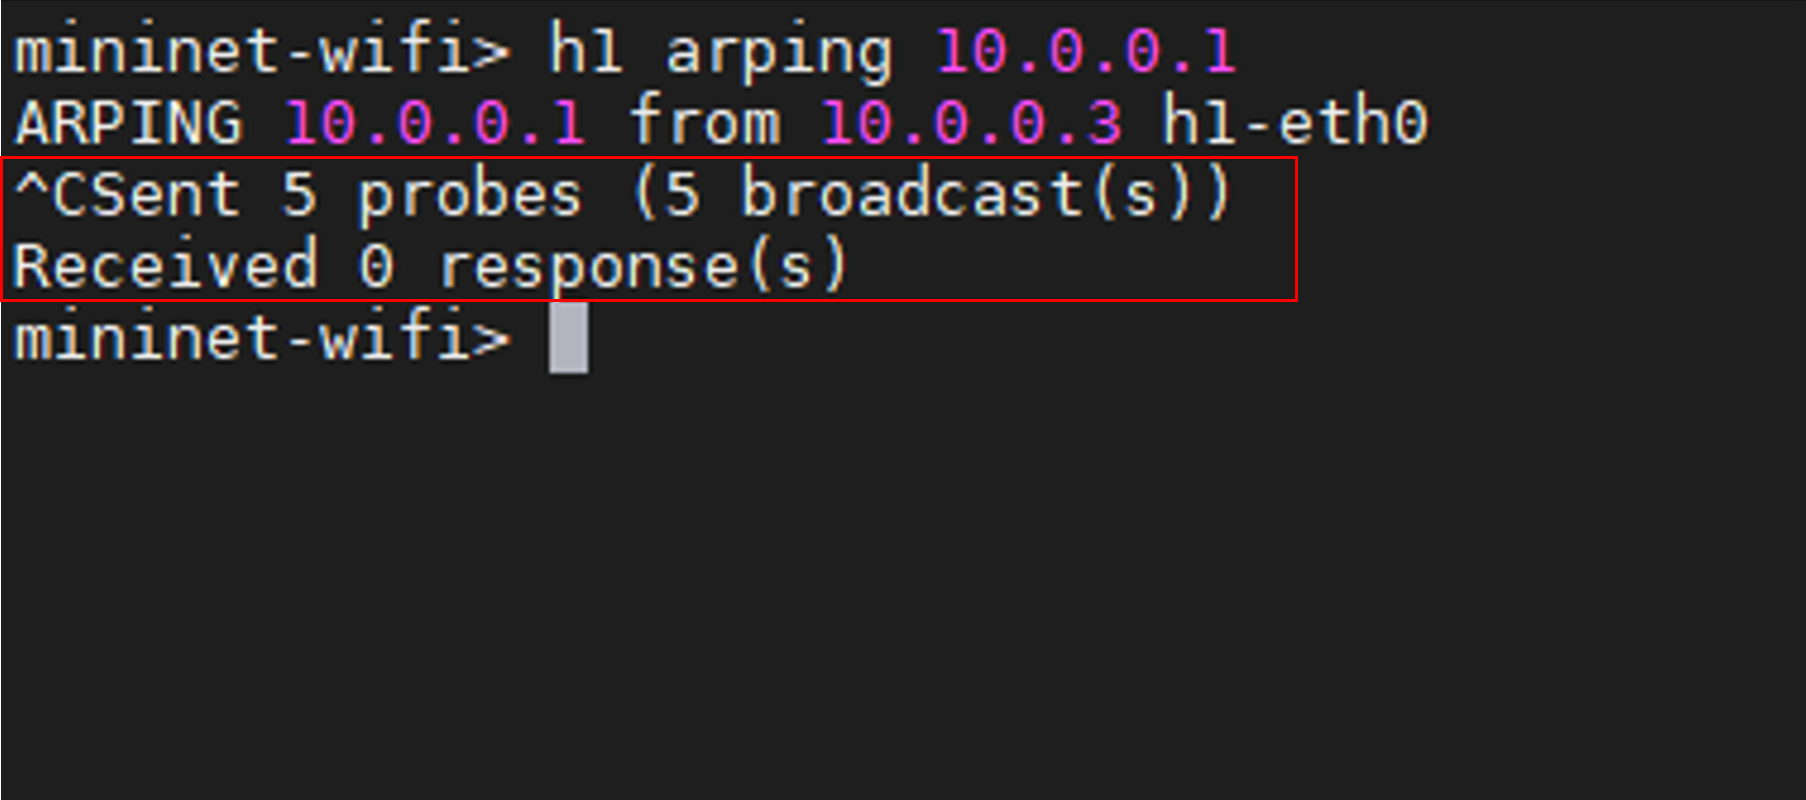
\includegraphics[width=7cm]{archivos/img/dev/xdp-wifi/case05/demo_case05_1_edited.png}
        \caption{Ejecución de arping hacia la estación WiFi sta1}
        \label{fig:case05_xdp_wifi_func_ping}
    \end{subfigure}
    \par\bigskip
    \begin{subfigure}[b]{\textwidth}
    	\centering
        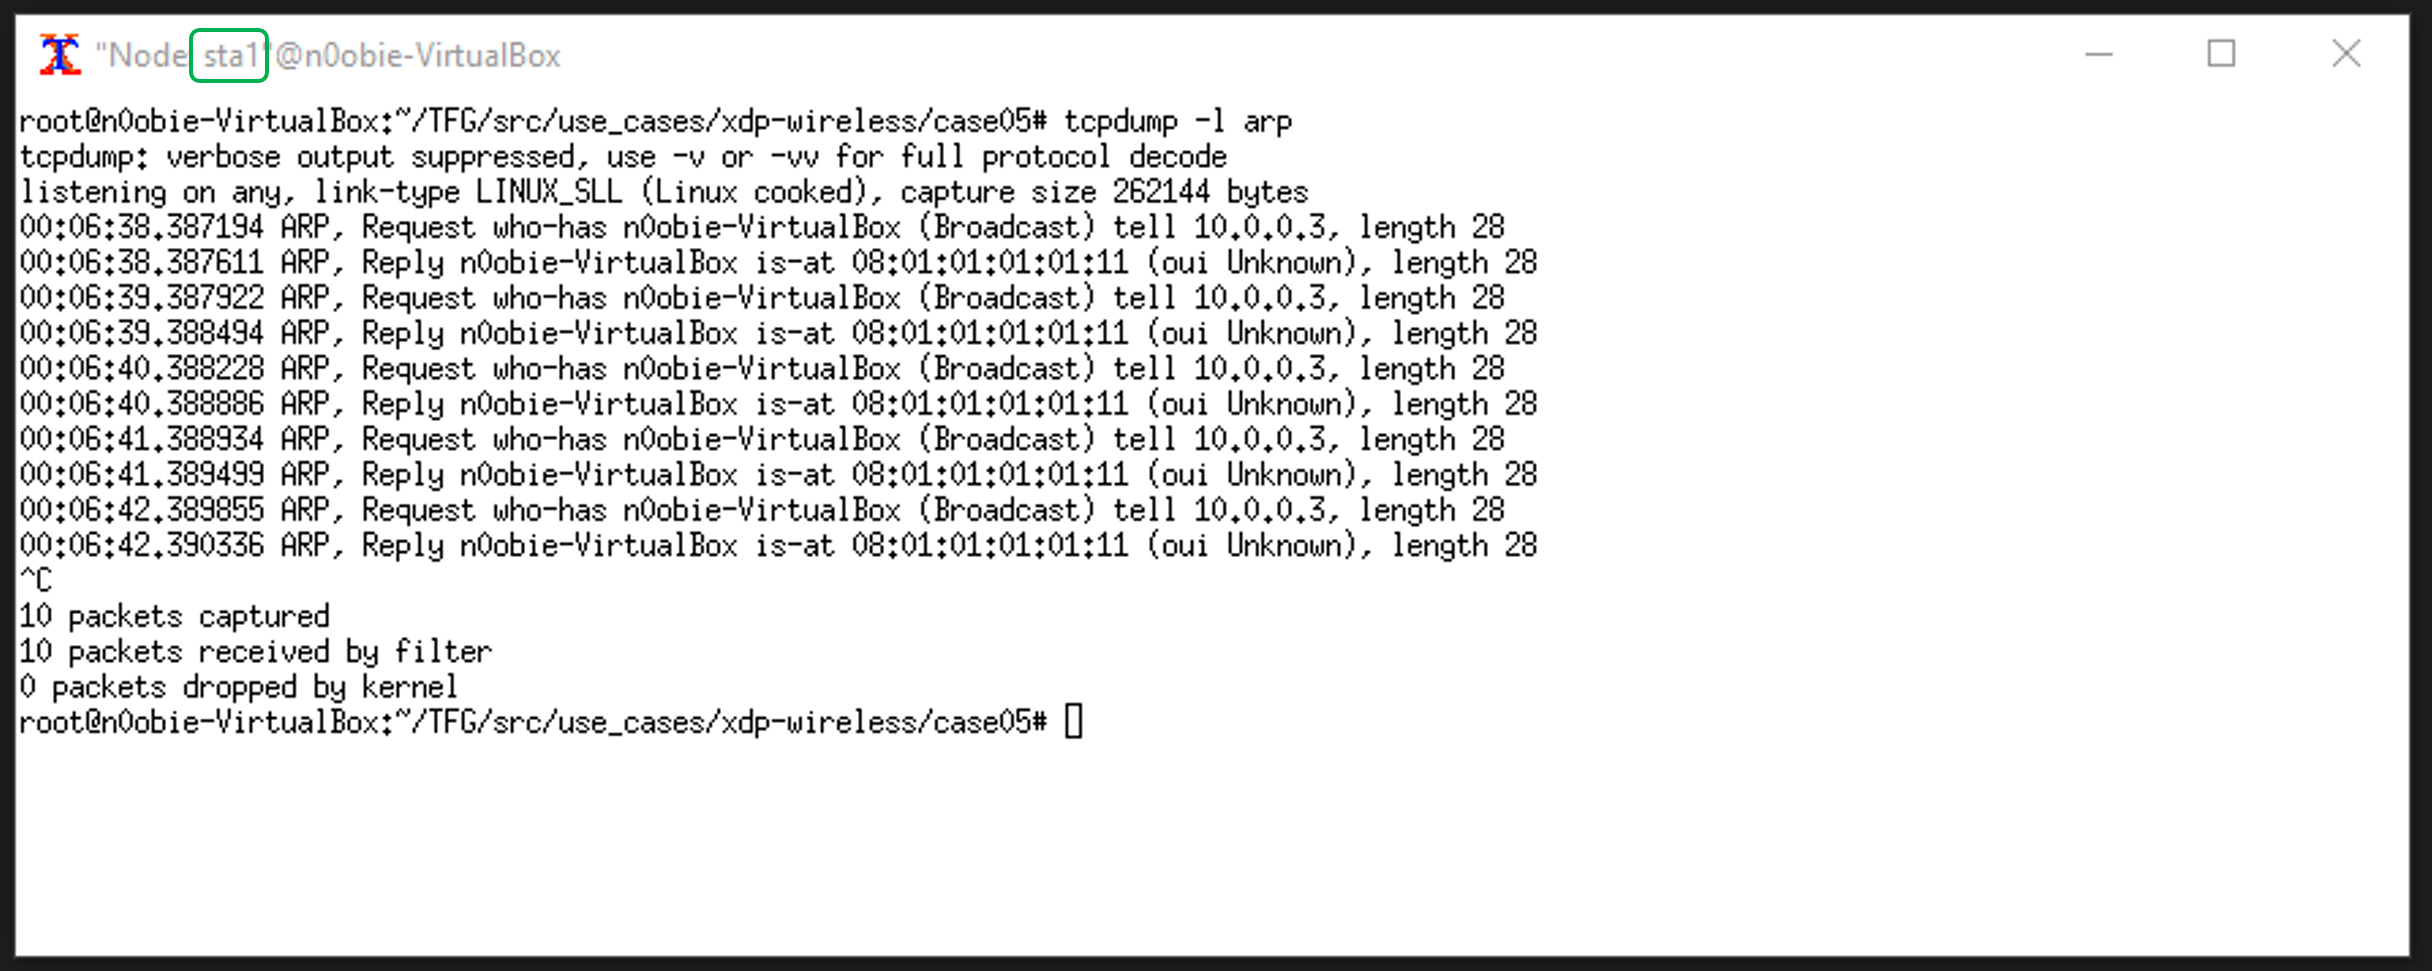
\includegraphics[width=14cm]{archivos/img/dev/xdp-wifi/case05/demo_case05_2_edited.png}
        \caption{Escucha con Tcpdump en la estación WiFi sta1}
        \label{fig:case05_xdp_wifi_func_list1}
    \end{subfigure}
    \par\bigskip
    \begin{subfigure}[b]{\textwidth}
    	\centering
        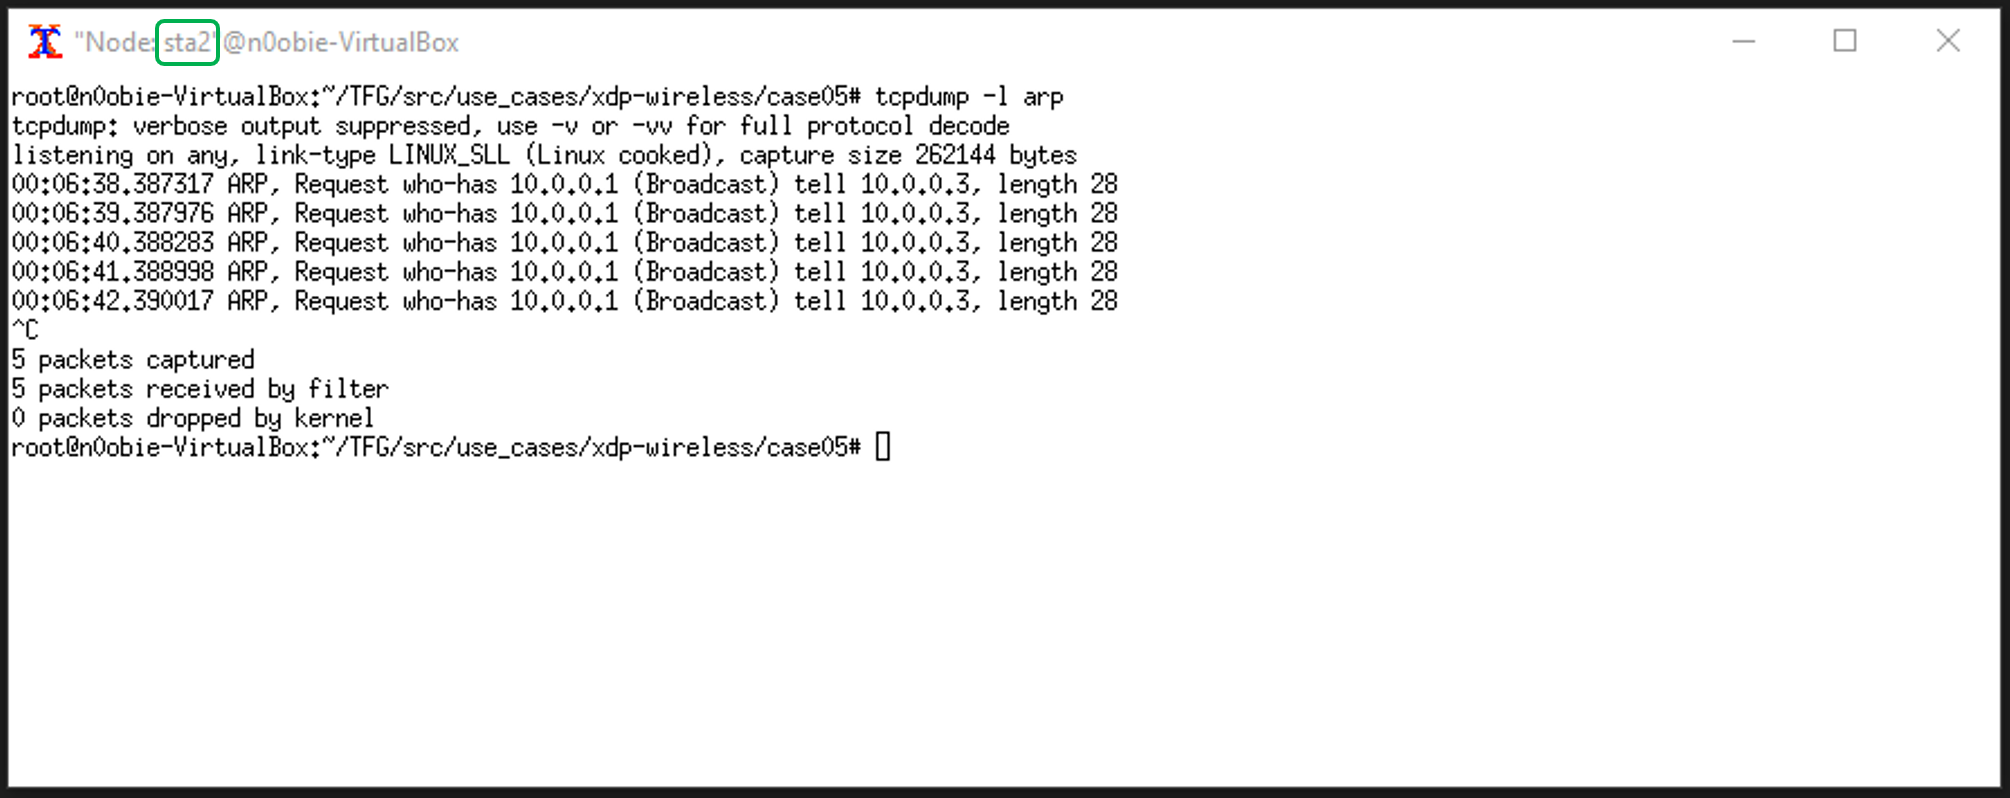
\includegraphics[width=14cm]{archivos/img/dev/xdp-wifi/case05/demo_case05_3_edited.png}
        \caption{Escucha con Tcpdump en la estación WiFi sta2}
        \label{fig:case05_xdp_wifi_func_list2}
    \end{subfigure}
    
    \caption{Comprobación de funcionamiento del Case05 - XDP Wireless}
    \label{fig:case05_xdp_wifi_func1}
\end{figure}


Como se puede apreciar en la figura \ref{fig:case05_xdp_wifi_func1}, ambas estaciones WiFi reciben el ARP-Request, siendo solo \texttt{sta1} quien conteste. La resolución ARP no se puede completar ya que no se ha implementado un sistema de forwarding en la \textit{Network Namespace} del \texttt{ap1}. Al igual que en el case05 (XDP Cableado \ref{xdp_ether_case05}), se propone hacer uso del los programas \gls{xdp} desarrollados en el caso de uso anterior para implementar un forwarding, y que así, las resoluciones se completasen. 


